% !TEX root=../main.tex

\section{The TopHat language}
\label{sec:tophat}

The Task-Oriented Programming (\TOP) paradigm was first introduced by Plasmeijer et al.~\cite{DBLP:conf/ppdp/PlasmeijerLMAK12}.
It is created to improve the development and quality of software that coordinates collaboration between users.
\TOP provides programmers with a high level of programming abstraction,
while still being expressive enough to describe real world collaborations.
It does so by using features from higher-order functional programming languages,
combined with the notion of \emph{tasks}.
Tasks model units of work, which can be performed by a human or by a computer.
From a task specification, a \TOP implementation generates a distributive multi-user (web) application.

Tasks have a couple of properties, listed below.
\begin{itemize}
  \item
    Tasks model \emph{collaboration}.\\
    Programmers describe what work needs to be done, by who and in what way.
  \item
    Tasks are \emph{interactive}.\\
    Users can enter or update information into the system by using \emph{editors}. They can progress to the next task, or choose between tasks.
  \item
    Tasks can be \emph{observed}.\\
    Therefore, other users or the system itself can make decisions based on the observed progress of the task.
  \item
    Tasks are \emph{modular}.\\
    They can be combined into bigger tasks by using \emph{combinators}.
    The basic combinators are chosen in such a way, that they represent basic collaboration patterns.
    New combinators can be created by making use of basic combinators and the (higher order) facilities of the host language.
  \item
    Tasks \emph{share information}.\\
    Information is passed along control flow, or via references to shared data, in order for tasks to exchange information.
  \item
    Tasks are \emph{typed}.\\
    This is not just to ensure safety at runtime,
    but also to automatically derive common program elements.
    \TOP systems automatically generate user interfaces and manage persistent storage of information.
\end{itemize}

Currently, there are three systems implementing the \TOP paradigm.
The reference implementation is the \ITASKS framework~\cite{DBLP:conf/ppdp/PlasmeijerLMAK12},
which is an embedded domain specific language in the non-strict functional programming language Clean~\cite{plasmeijer2002clean}.
\MTASKS~\cite{DBLP:conf/cgo/KoopmanLP18} is a \TOP implementation specifically designed for embedded systems.
A formalisation of \TOP, called \TOPHAT (TopHat), has been created by Steenvoorden, Naus, and Klinik~\cite{DBLP:conf/ppdp/SteenvoordenNK19}.
Assistive \TOPHAT builds on \TOPHAT and its symbolic counterpart \STOPHAT~\cite{Naus2019}.

\TOPHAT implements \TOP by embedding a task language in the simply typed lambda calculus with references, conditionals, and pairs.
\STOPHAT extends this with built in operators, lists, and most importantly symbols.
References are used to model the shared data component of \TOP.
The complete syntax and semantics can be found in previous work~\cite{DBLP:conf/ppdp/SteenvoordenNK19}.
In the next subsections we describe the basic constructs of the \TOPHAT language.
\cref{sec:symbolic} details \STOPHAT.


\subsection{Editors}

Editors form the entry points for interaction and communication with the outside world.
They are the most basic tasks and can be seen as an abstraction over widgets in a \GUI library or forms on a webpage.
Users can change the value held by an editor, in the same way they can manipulate widgets in a \GUI.

When a \TOP implementation generates an application from a task specification, it derives user interfaces for the editors.
The appearance of an editor depends on its type.
For example, editors of type strings can be represented by simple input fields, dates by calendars, and locations by pins on a map.

There are three different editors in \TOPHAT.
\begin{description}
  \item[$\Edit v$] Valued editor.\\
    This editor holds a value $v$ of a certain type.
    The user can replace the value by new values of the same type.
  \item[$\Enter \tau$] Unvalued editor.\\
    This editor holds no value, and can receive a value of type $\tau$.
    When that happens, it turns into a valued editor.
  \item[$\Update l$] Shared editor.\\
    This editor refers to a store location $l$.
    Its observable value is the value stored at that location.
    When it receives a new value, this value will be stored at location $l$.
\end{description}


\subsection{Combinators}

Editors can be combined into larger tasks using combinators.
The order in which editors and tasks are executed is specified with combinators. Tasks can be performed in sequence, in parallel or a choice can be made between tasks.


The following combinators are available in \TOPHAT.
Here, $t$ stands for tasks and $e$ for expressions.
\begin{description}
  \item[$t \Then e$] Step.\\
    Users can work on task $t$.
    As soon as $t$ has an observable value, as defined in the next section, that value is passed on to the right hand side $e$.
    The expression $e$ is a function, taking the value as an argument, resulting in a new task.
  \item[$t \Next e$] User Step.\\
    Users can work on task $t$.
    When $t$ has an observable value, the step becomes enabled.
    Then, users can send a continue event to the combinator.
    When that happens, the value of $t$ is applied to the right hand side function $e$, with which it continues,
    in the same way as normal steps do.
  \item[$t_1 \And t_2$] Pair.\\
    Users can work on tasks $t_1$ and $t_2$ in at the same time.
  \item[$t_1 \Or t_2$] Choice.\\
    The system chooses between $t_1$ or $t_2$,
    based on which task first has an observable value.
    If both tasks have a value, the system chooses the left one.
    When neither of the two tasks has an observable value, users can continue to work on both tasks until one of them does.
  \item[$e_1 \Xor e_2$] User choice.\\
    A user has to make a choice between either the left or the right hand side.
    After picking a side, the user can work on that task.
\end{description}

In addition to editors and combinators, \TOPHAT also contains the fail task ($\Fail$).
Programmers can use this task to indicate that a task is not reachable or viable.
When the right hand side of a step combinator evaluates to $\Fail$, the step will not proceed to that task.


\subsection{Observations}

Several observations can be made on tasks.
These observations are used by the system to determine the progress of combinators,
to draw the user interface, and they will also be used by Assistive \TOPHAT to provide next step hints.

Using the value function $\Value$, the current value of a task can be determined.
The value function is a partial function, since not all tasks have a value.
For example empty editors do not have a value.
The value of tasks composed of parallel and internal choice combinators, depends on the value of the subtasks.
Parallel only has a value if both tasks have an observable value.
Internal choice has a value if either of the two tasks has an observable value.

One can also observe whether or not a task is failing, by means of the failing function $\Failing$.
A task is considered to be failing if, after normalisation, a user cannot interact with it.
For example, the valued editor is not failing, since the user can update it with a new value.
The task $\Fail$ is failing, as is a parallel combination of failing tasks $\Fail \And \Fail$, since both the left and the right task cannot be interacted with.
Both observation definitions can be found in \cref{fig:observations}

\begin{figure}[h]
  \begin{minipage}{\textwidth}
    \centering \small
    \usemacro{O-Value}  \usemacro{O-Failing}
  \end{minipage}
  \caption{
    Observations on task $t$.
    $\Value$ gets the value of $t$, $\Failing$ observes if it is unsafe to step to $t$.
    Note that $\Value$ is a partial function.
  }
  \label{fig:observations}
\end{figure}

The step combinator makes use of both functions in order to determine if it can step.
First, it uses $\Value$ to see if the left hand side produces a value.
If that is the case, it uses the $\Failing$ function to see if stepping to the right hand side is successful.


\subsection{Input}

Input events drive the evaluation of tasks.
Because tasks are typed, input is typed as well.
Editors only accept input of the correct type.
For example, an editor can only be updated with a new value, if it has the same type as the old value.
When the system receives a valid event, it applies this event to the current task, which evaluates to a new task.
Everything in between two events is evaluated atomically with respect to inputs.
This means that tasks are normalised up to the point where they await new user interactions.
% In this way the system communicates with the environment.

Input events are synchronous, which means that the order of execution is completely determined by the order of the events.
In particular, the order of input events determine the progression of parallel branches.


\subsection{Semantics}

\begin{figure}[h]
\centering
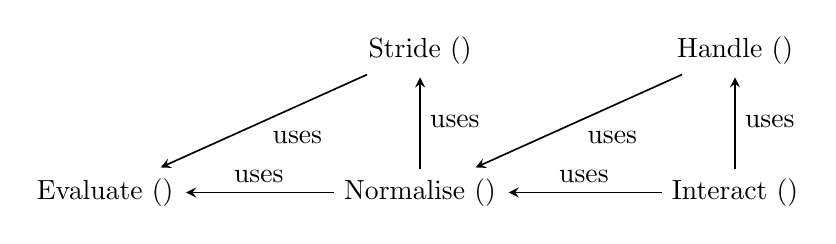
\begin{tikzpicture}[
            > = stealth, % arrow head style
            shorten > = 1pt, % don't touch arrow head to node
            auto,
            node distance = 3cm, % distance between nodes
            semithick, % line style
        ]

        \node (interact)  {Interact ($\interact{}$)};
        \node (handle) [above of=interact,yshift=-1.2cm] {Handle ($\handle{}$)};
        \node (normalise) [left of=interact,xshift=-1cm] {Normalise ($\normalise$)};
        \node (stride) [left of=handle,xshift=-1cm] {Stride ($\stride$)};
        \node (evaluate) [left of=normalise,xshift=-1cm] {Evaluate ($\eval$)};


        \path[->,right] (interact) edge node {uses} (handle);
        \path[->,above] (interact) edge node {uses} (normalise);

        \path[->] (handle) edge node {uses} (normalise);

        \path[->,right] (normalise) edge node {uses} (stride);
        \path[->,above] (normalise) edge node {uses} (evaluate);

        \path[->] (stride) edge node {uses} (evaluate);

    \end{tikzpicture}
    \caption{
      Semantic functions defined in this report and their relation.
    }
    \label{fig:semantic-functions}
  \end{figure}
